\chapter{Теоретичні дослідження}
\section{Попередня робота}
Трансформери були запропоновані \cite{attention-all-need}
для машинного перекладу, і з тих пір стали
найсучаснішим методом у багатьох задачах обробки природної
мови. Великі моделі на основі трансформерів
часто попередньо навчаються на великих корпусах, а потім
доопрацьовуються для виконання поставленого завдання:
BERT \cite{bert}, GPT \cite{gpt}.

У попередніх роботах були запропоновані методи, які об'єднують
рекурентні і згорткові шари в одній моделі, для виконання задач
багатоміткової класифікації \cite{nn:cnn-rnn}, опису зображень.
Трансформери завдяки механізму уваги можуть
замінити рекурентні та згорткові шари. Наївне застосування
уваги до зображень вимагало б, щоб кожен піксель приділяв
увагу кожному іншому пікселю. При квадратичній вартості відносно кількості
пікселів, це не практично щодо реальних розмірів
вхідних зображень. Таким чином, щоб застосувати
трансформери в контексті обробки зображень,
раніше було спробувано кілька наближень. Одним з них
було застосовування самоуваги лише в локальних
регіонах для кожного пікселя запиту, а не глобально \cite{image-trans}.
Такі локальні багатоголовкові блоки із самоувагою
можуть повністю замінити згортання \cite{local-regions-attention}.

Найбільш пов’язаною з нашою є модель \cite{cordonnier},
яка розділяє вхідне зображення на регіони розміром
$2 \times 2$ і зверху застосовує повну увагу. Ця робота
дуже схоже на нашу, проте наша робота йде далі,
демонструючи, що масштабна попереднє тренування
робить звичайні трансформери
конкурентоспроможними (або навіть кращими) із найсучаснішими ЗНМ.
Також, \cite{cordonnier} використовує маленький розмір
регіону $2 \times 2$, що не дозволяє використовувати модель
на занадто великих зображеннях, коли наша модель успішно обробляє
зображення середнього розміру.

\section{Метод}

При розробці моделі ми максимально точно дотримуємося
оригінального трансформера \cite{attention-all-need}.
Перевагою цього навмисно простого підходу
є те, що масштабовані архітектури трансформерів
для задач обробки природної мови (та їх ефективні реалізації)
можуть бути використані майже без модифікацій.

\begin{figure}[H]
    \centering
    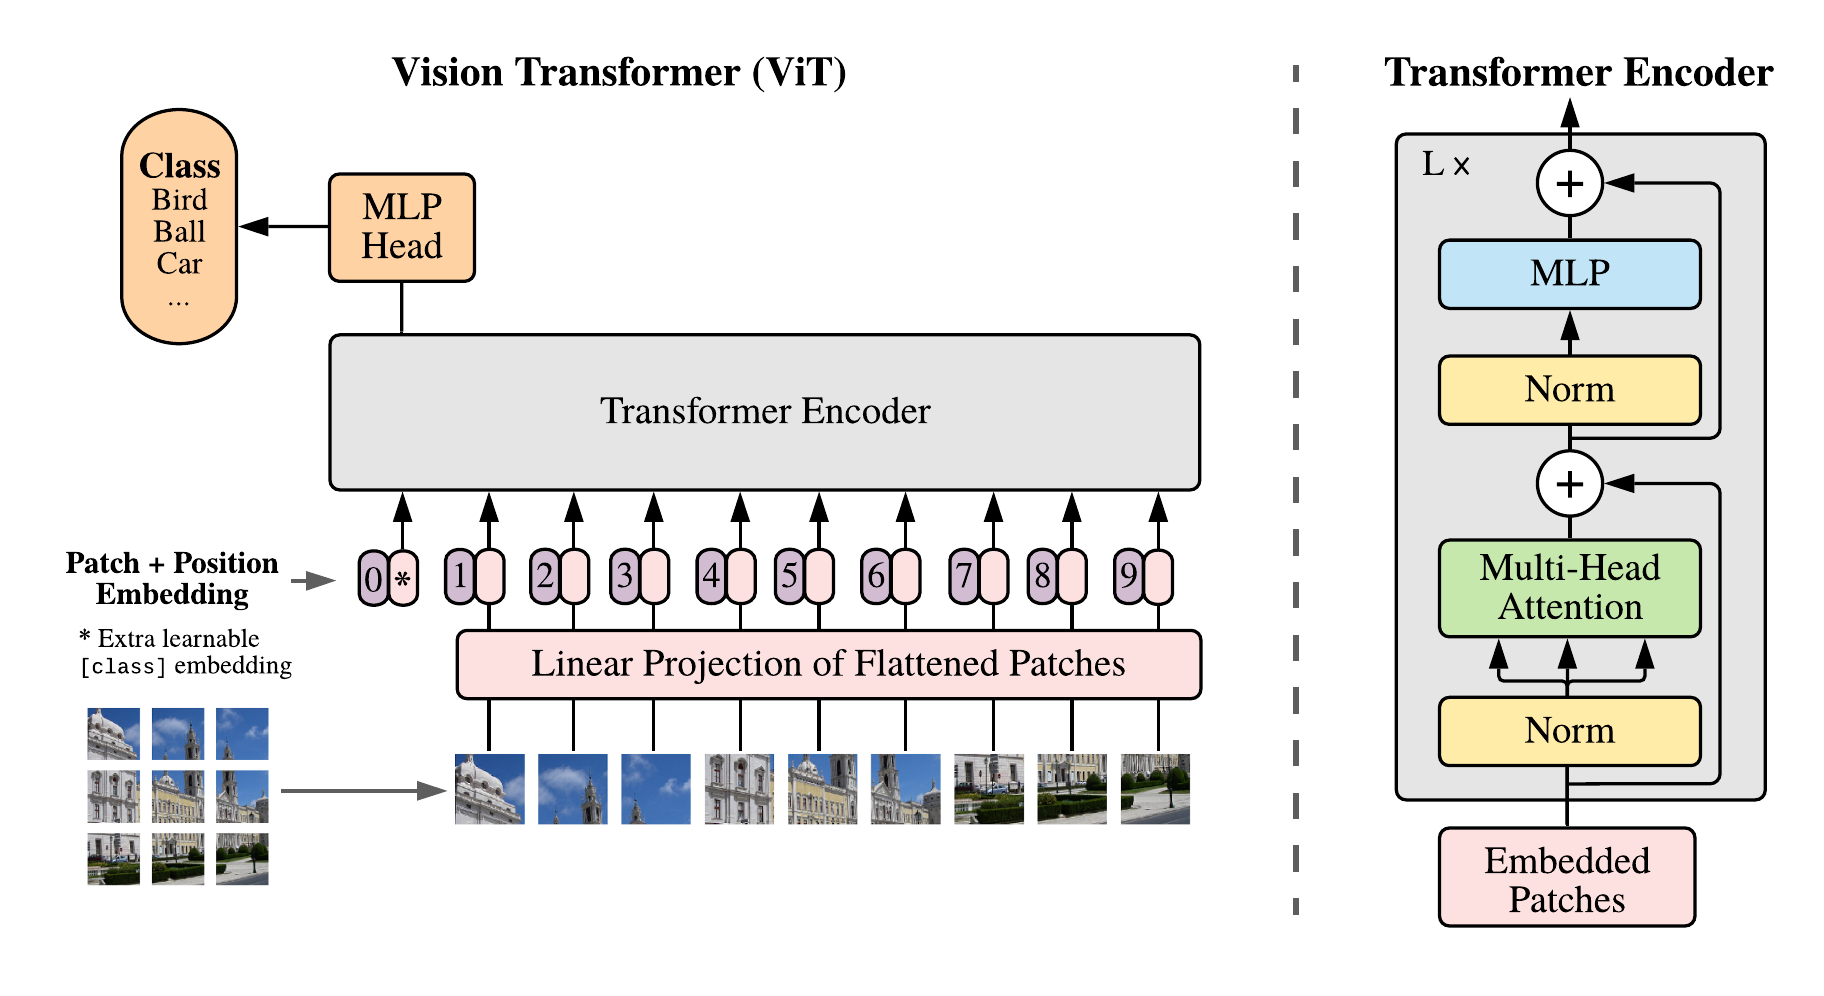
\includegraphics[width=1\textwidth]{vision-transformer-arch.png}
    \caption{Архітектура моделі}
    \label{fig:model-arch}
\end{figure}

\subsection{Vision Transformer}
Огляд моделі наведено на рисунку \ref{fig:model-arch}.
Стандартний трансформатор отримує на вхід 1D
послідовність ембедингів токенів.
Для обробки 2D-зображень ми змінюємо розмірність зображення
$x \in \mathbb{R}^{H\times W \times C}$ у послідовність
зплющених 2D регіонів $x_p \in \mathbb{R}^{N\times (P^2\cdot C)}$,
де $(H, W)$ -- роздільна здатність початкового
зображення, $C$ -- кількість каналів, $(P, P)$ -- роздільна
здатність кожного регіону зображення,
а $N = HW / P^2$ -- результуюча кількість регіонів,
яка також служить ефективною довжиною вхідної послідовності для
трансформера.

\section{Модель}
% In order to perform classification, we use the standard approach of adding an extra learnable “classification token” to the sequence.
% https://stackoverflow.com/questions/58123393/how-to-use-transformers-for-text-classification